\chapter{General description}
\thispagestyle{fancy}
\minitoc[n] % Creating an actual minitoc

\section{General}
This pilot's operating handbook is designed  to provide information relevant to achieve maximum utilisation 
of the aircraft.  It is not designed to be a substitute for adequate and competent flying instruction 
and should not be used for operational purposes unless kept up to date.

Assurance that the aircraft is airworthy is the responsibility of the owner.  The pilot in command is responsible for
ensuring the aircraft is safe for flight and for operating within the limits detailed in this handbook and as displayed on placards and instrument markings in the aircraft.

\section{Three View}
The RV7 is a propeller driven conventional gear aircraft with a wingspan of 7.7m, a length of 6.1m and a height of 1.6m as shown in Figure~\ref{fig:rv-7_3view}.

\begin{figure}[H]
\centering
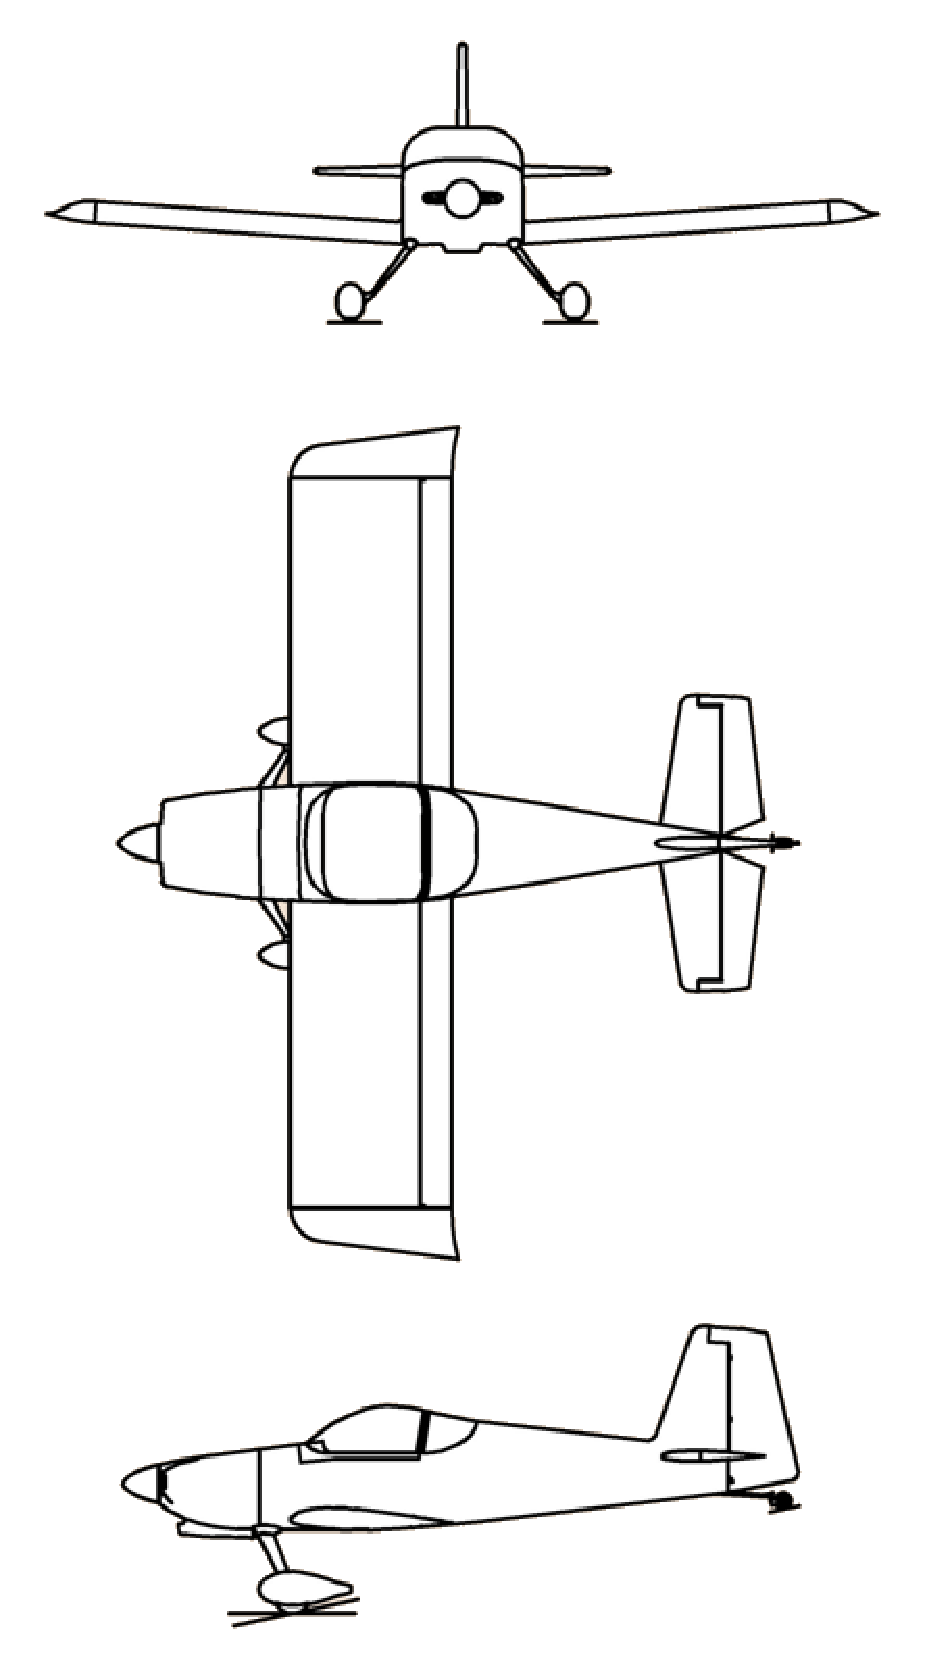
\includegraphics[height=0.5\textheight]{rv-7_3view.eps}
\caption{RV7 three view: Wingspan 7.7m, Length 6.1m, Height 1.6m}
\label{fig:rv-7_3view}
\end{figure}

\section{Descriptive Data}
\subsection{Engine}
%Four cylinder air-cooled, horizontally opposed, direct drive, fuel injected, tuned induction engine having oil jets for internal piston cooling.  Provisions for single action controllable pitch propeller.  Impulse coupling magnetos.  Crankshaft equipped with one 6.3 order and one 8th order counterweights.

\begin{tabularx}{\linewidth}{
  >{\hsize=0.4\hsize}X
  >{\hsize=0.6\hsize}X  }
 Number of Engines: & 1  \\ 
 Engine manufacturer: & Avco Lycoming  \\  
 Engine Type: & Normally-aspirated, air-cooled, horizontally opposed, fuel injected, four-cylinder engine\\
 Engine Model number: & IO-360-A1B6\\
 Rated horespower: & 200 hp\\
 Rated speed, RPM: & 2700 rpm \\
 Displacement, cu inch: & 361.0\\
 Compression ratio: & 8.7:1 \\
 Firing order: & 1-3-2-4 \\
 Spark plugs: & Champion REM38E or REB37E \\
 Propeller rotation: & Clockwise \\
 Weight: & 333 lbs \\

\end{tabularx}

\subsection{Propeller}
  \begin{tabularx}{\linewidth}{
    >{\hsize=0.4\hsize}X
    >{\hsize=0.6\hsize}X  }
Propeller Manufacturer: & Hartzell\\
Propeller Model No: & HC-C2YR-1BFP/F7497-2\\%HC - Hartzell controllable, C2YR C-Standard Hub, 2 - no. of blades, YR - Y shank aluminium blade, R - mounting flange, 
%1 CONSTANT SPEED, NO COUNTERWEIGHT OIL PRESSURE TO HIGH PITCH, BLADE CENTRIFUGAL FORCE TO LOW
%BFP B-830-21 STOP UNITS F-LARGE PITCH CHANGE KNOB, FORK
%F - large pitch change knob Y shank 
%74 - blade diameter next number spec model. 
Number of Blades: & 2\\
Propeller Diameter: & Maximum 72"\\ %% I believe we can say 72" here as it is exactly that.
Propeller Type: & Variable Pitch\\
Weight: & 51.8 lbs \\
Limitation: & None\newline (Type Certificate Data sheet No. P-920)\\
\end{tabularx}

\subsection{Fuel}
  \begin{tabularx}{\linewidth}{
    >{\hsize=0.4\hsize}X
    >{\hsize=0.6\hsize}X  }
Approved Fuel Grades: & 100/130 Aviation Fuel (Blue).\\
Capacity: & 42 US Gal (159$\ell$)\\
Useable fuel: & 40 US Gal (151$\ell$)\\ % Could be as high as 41.94 but should be measured
Max fuel pressure: & 12psi (CHECK THIS)\newline  (>9psi indicates possible blocked injector)\\
\end{tabularx}

\subsection{Oil}
  \begin{tabularx}{\linewidth}{
    >{\hsize=0.4\hsize}X
    >{\hsize=0.6\hsize}X  }
Oil capacity: & 8 US Qt (min 2 US Qt) \\
\end{tabularx}

\subsection{Maximum Weights}
  \begin{tabularx}{\linewidth}{
    >{\hsize=0.4\hsize}X
    >{\hsize=0.6\hsize}X  }
Maximum weight: & 1800 lbs (820 kg)\\
Max baggage weight: & 100 lbs (45 kg) \\

\end{tabularx}

\subsection{Standard airplane weights}
  \begin{tabularx}{\linewidth}{
    >{\hsize=0.4\hsize}X
    >{\hsize=0.6\hsize}X  }
Standard empty weight: & 1122 lbs (510 kg)\\
Usable load: & 679 lbs (310kg) \\
\end{tabularx}

\subsection{Cabin and Entry dimensions}
The cabin features side by side seating with control and  brakes for both occupants.   Cabin entry is made through the open canopy by stepping from the wing over the cabin side onto the seat.

\subsection{Baggage space and entry dimensions}
Baggage is stored behind the seatbacks of the front occupants.  A maximum weight of 100 lbs and volume of 12 cubic feet is available for baggage.

\subsection{Specific loadings}
  \begin{tabularx}{\linewidth}{
    >{\hsize=0.4\hsize}X
    >{\hsize=0.6\hsize}X  }
Wing Loading: & 14.8 lb/sq ft\\
Power Loading: & 9.0 lb/hp \\
\end{tabularx}

\section{Symbols}
  \begin{tabularx}{\linewidth}{
    >{\hsize=0.2\hsize}X
    >{\hsize=0.8\hsize}X  }
$V_{a}$    & Manoeuvring speed. Speed at which full application of aerodynamic control will not overstress the aircraft. \\
$V_{fe}$ & Maximum Flap Extension Speed. Highest Speed permissible with wing flaps in a prescribed extended position. \\
$V_{ne}$ & Never exceed speed. Not to be exceeded at any time. \\
$V_{no}$ & Maximum structural cruising speed. Not to be exceeded except in smooth air and then only with caution.\\ 
$V_{s}$  & Stalling speed. The minimum steady airspeed at which the aircraft is controllable. \\
$V_{so}$ & Stalling speed. The minimum steady airspeed at which the aircraft is controllable, in the landing configuration. \\
$V_{x}$  & Best angle of climb. Airspeed that delivers greatest altitude gain in shortest horizontal movement. \\
$V_{y}$  & Best rate of climb. Airspeed delivering greatest altitude gain in shortest possible time.\\
$V_{gl}$ & Best glide speed for lowest sink rate. (propeller set to fine)\\
\end{tabularx}

\section{Abbreviations}
  \begin{tabularx}{\linewidth}{
    >{\hsize=0.2\hsize}X
    >{\hsize=0.8\hsize}X  }
CAS & Calibrated airspeed. Indicated airspeed corrected for position and instrument error. Equates to true airspeed in standard atmosphere at sea level. \\
%KCA & CAS in” Knots” \\
GS & Groundspeed. Speed relative to the ground \\
IAS & Indicated Airspeed. Speed, as shown on Airspeed indicator, includes instrument and position error. \\
KIAS & IAS in Knots \\
kt & Knots \\
NM & Nautical Miles\\
TAS & True airspeed relative to undisturbed air, which is the CAS, corrected for altitude, temperature and pressure. \\
\end{tabularx}

\section{Terminology}
  \begin{tabularx}{\linewidth}{
    >{\hsize=0.2\hsize}X
    >{\hsize=0.8\hsize}X  }
%Accelerate-Stop Distance: & Distance to accelerate to a specified speed and, assuming engine failure when that speed is attained, bring the aircraft to a stop. \\
Constant Speed & A propeller system which employs a governing device to maintain a selected engine RPM.\\
Demonstrated crosswind & Demonstrated cross wind component for which adequate control of the aircraft during take off and landing has been demonstrated.\\
Empty Weight & Weight of the airplane including fixed ballast, unusable fuel and oil.\\
Gross Weight & Sum of empty weight plus crew, passengers, fuel and baggage.  \\
Maximum Gross Weight & The maximum allowable operating weight with all variable load items located such that the Centre of Gravity remains within prescribed limits.\\
Payload & Weight of passengers and baggage.\\
Useful Load & Weight of passengers, fuel and baggage.\\
\end{tabularx}

